%%%%%%%%%%%%%%%%%%%%%%%%%%%%%%%%%%%%%%%%%
% Beamer Presentation
% LaTeX Template
% Version 2.0 (March 8, 2022)
%
% This template originates from:
% https://www.LaTeXTemplates.com
%
% Author:
% Vel (vel@latextemplates.com)
%
% License:
% CC BY-NC-SA 4.0 (https://creativecommons.org/licenses/by-nc-sa/4.0/)
%
%%%%%%%%%%%%%%%%%%%%%%%%%%%%%%%%%%%%%%%%%

%----------------------------------------------------------------------------------------
%	PACKAGES AND OTHER DOCUMENT CONFIGURATIONS
%----------------------------------------------------------------------------------------

\documentclass[
	11pt, % Set the default font size, options include: 8pt, 9pt, 10pt, 11pt, 12pt, 14pt, 17pt, 20pt
	% t, % Uncomment to vertically align all slide content to the top of the slide, rather than the default centered
	aspectratio=169, % Uncomment to set the aspect ratio to a 16:9 ratio which matches the aspect ratio of 1080p and 4K screens and projectors
]{beamer}
\graphicspath{{./images/}} % Specifies where to look for included ./images (trailing slash required)

\usepackage{booktabs} % Allows the use of \toprule, \midrule and \bottomrule for better rules in tables

\usepackage[T1]{fontenc}
\usepackage[utf8]{inputenc}
\usepackage{hyperref}

%----------------------------------------------------------------------------------------
%	SELECT LAYOUT THEME
%----------------------------------------------------------------------------------------

% Beamer comes with a number of default layout themes which change the colors and layouts of slides. Below is a list of all themes available, uncomment each in turn to see what they look like.

%\usetheme{default}
%\usetheme{AnnArbor}
%\usetheme{Antibes}
%\usetheme{Bergen}
%\usetheme{Berkeley}
%\usetheme{Berlin}
%\usetheme{Boadilla}
%\usetheme{CambridgeUS}
%\usetheme{Copenhagen}
%\usetheme{Darmstadt}
%\usetheme{Dresden}
%\usetheme{Frankfurt}
%\usetheme{Goettingen}
%\usetheme{Hannover}
%\usetheme{Ilmenau}
%\usetheme{JuanLesPins}
%\usetheme{Luebeck}
\usetheme{Madrid}
%\usetheme{Malmoe}
%\usetheme{Marburg}
%\usetheme{Montpellier}
%\usetheme{PaloAlto}
%\usetheme{Pittsburgh}
%\usetheme{Rochester}
%\usetheme{Singapore}
%\usetheme{Szeged}
%\usetheme{Warsaw}

%----------------------------------------------------------------------------------------
%	SELECT COLOR THEME
%----------------------------------------------------------------------------------------

% Beamer comes with a number of color themes that can be applied to any layout theme to change its colors. Uncomment each of these in turn to see how they change the colors of your selected layout theme.

%\usecolortheme{albatross}
%\usecolortheme{beaver}
%\usecolortheme{beetle}
%\usecolortheme{crane}
%\usecolortheme{dolphin}
%\usecolortheme{dove}
%\usecolortheme{fly}
%\usecolortheme{lily}
%\usecolortheme{monarca}
%\usecolortheme{seagull}
%\usecolortheme{seahorse}
%\usecolortheme{spruce}
%\usecolortheme{whale}
%\usecolortheme{wolverine}

%----------------------------------------------------------------------------------------
%	SELECT FONT THEME & FONTS
%----------------------------------------------------------------------------------------

% Beamer comes with several font themes to easily change the fonts used in various parts of the presentation. Review the comments beside each one to decide if you would like to use it. Note that additional options can be specified for several of these font themes, consult the beamer documentation for more information.

\usefonttheme{default} % Typeset using the default sans serif font
%\usefonttheme{serif} % Typeset using the default serif font (make sure a sans font isn't being set as the default font if you use this option!)
%\usefonttheme{structurebold} % Typeset important structure text (titles, headlines, footlines, sidebar, etc) in bold
%\usefonttheme{structureitalicserif} % Typeset important structure text (titles, headlines, footlines, sidebar, etc) in italic serif
%\usefonttheme{structuresmallcapsserif} % Typeset important structure text (titles, headlines, footlines, sidebar, etc) in small caps serif

%------------------------------------------------

%\usepackage{mathptmx} % Use the Times font for serif text
\usepackage{palatino} % Use the Palatino font for serif text

%\usepackage{helvet} % Use the Helvetica font for sans serif text
\usepackage[default]{opensans} % Use the Open Sans font for sans serif text
%\usepackage[default]{FiraSans} % Use the Fira Sans font for sans serif text
%\usepackage[default]{lato} % Use the Lato font for sans serif text

%----------------------------------------------------------------------------------------
%	SELECT INNER THEME
%----------------------------------------------------------------------------------------

% Inner themes change the styling of internal slide elements, for example: bullet points, blocks, bibliography entries, title pages, theorems, etc. Uncomment each theme in turn to see what changes it makes to your presentation.

%\useinnertheme{default}
\useinnertheme{circles}
%\useinnertheme{rectangles}
%\useinnertheme{rounded}
%\useinnertheme{inmargin}

%----------------------------------------------------------------------------------------
%	SELECT OUTER THEME
%----------------------------------------------------------------------------------------

% Outer themes change the overall layout of slides, such as: header and footer lines, sidebars and slide titles. Uncomment each theme in turn to see what changes it makes to your presentation.

%\useoutertheme{default}
%\useoutertheme{infolines}
%\useoutertheme{miniframes}
%\useoutertheme{smoothbars}
%\useoutertheme{sidebar}
%\useoutertheme{split}
%\useoutertheme{shadow}
%\useoutertheme{tree}
%\useoutertheme{smoothtree}

%\setbeamertemplate{footline} % Uncomment this line to remove the footer line in all slides
%\setbeamertemplate{footline}[page number] % Uncomment this line to replace the footer line in all slides with a simple slide count
%\setbeamertemplate{navigation symbols}{} % Uncomment this line to remove the navigation symbols from the bottom of all slides
% set \caption's to exclude prefixes, e.g. 'Figure: ...'
\setbeamertemplate{caption}{\raggedright\insertcaption\par}
% \setbeameroption{show notes on second screen} % hidden notes with \note

%----------------------------------------------------------------------------------------
%	PRESENTATION INFORMATION
%----------------------------------------------------------------------------------------

% The short title in the optional parameter appears at the bottom of every slide, the full title in the main parameter is only on the title page
\title[INF-2200]{INF-2200}

% Presentation subtitle, remove this command if a subtitle isn't required
\subtitle{Introduction to Assembly}

% Presenter name(s), the optional parameter can contain a shortened version to appear on the bottom of every slide, while the main parameter will appear on the title slide
\author[\O yvind \and Ragnhild \and J\o rgen \and Vi \and  Lars ]{N.M. \O yvind \and G.A. Ragnhild \and O.K. J\o rgen  \and T.N. Vi\and Lars Ailo Bongo } 

% Your institution, the optional parameter can be used for the institution shorthand and will appear on the bottom of every slide after author names, 
% while the required parameter is used on the title slide and can include your email address or additional information on separate lines
\institute[UiT]{University of Troms\o \\ \smallskip  \textit{oyvind.a.nohr@uit.no} \textit{ragnhild.a.grape@uit.no} \textit{jorgen.k.olsen@uit.no}\\
\textit{vi.n.tran@uit.no} \textit{lars.ailo.bongo@uit.no}} 

% Presentation date or conference/meeting name, the optional parameter can contain a shortened version to appear on the bottom of every slide, while the required parameter value is output to the title slide
\date[\today]{Computer Architecture \\ \today}
%----------------------------------------------------------------------------------------

\begin{document}

%----------------------------------------------------------------------------------------
%	TITLE SLIDE
%----------------------------------------------------------------------------------------
\begin{frame} % {no title}

    % Output the title slide, automatically created using the text entered in the PRESENTATION INFORMATION block above
    \titlepage
    % Present presenters

\end{frame}
\begin{frame}[allowframebreaks]{Overview} % ??use after each presentation section??

    % Output the table of contents (all sections on one slide)
    \tableofcontents

    % Output the table of contents (break sections up across separate slides)
    % \tableofcontents[pausesections]

    % The table of contents outputs the sections and subsections that appear in your presentation, 
    % specified with the standard \section and \subsection commands. 
    % You may either display all sections and subsections on one slide with \tableofcontents, 
    % or display each section at a time on subsequent slides with \tableofcontents[pausesections]. 
    % The latter is useful if you want to step through each section and mention what you will discuss.

\end{frame}

%----------------------------------------------------------------------------------------
%	PRESENTATION BODY SLIDES
%----------------------------------------------------------------------------------------
\section{Introduction}
\def \sectiontitle{Instruction set architecture}
\begin{frame}\Huge{\underline{\sectiontitle} (ISA)}\end{frame}
\subsection{ISA: x86-64}
\def \sectiontitle{ISA}
\begin{frame}{ISA: x86-64}{\sectiontitle}

    \begin{columns}
        \column{\textwidth}
        \textbf{ISA}
        \begin{itemize}
            \item An ISA enables multiple different hardware to implement the same functionality in different ways. That is why you can play your games on both AMD and Intel processors
            \item We will focus on the \textbf{x86-64} ISA, but there exist many more and perhaps most used is the \textbf{ARM}-family
            \item As we know from previous courses, memory can be viewed as a collection of \underline{bits}
            \item This ISA can only access \textbf{groups} of bits at a time
            \item  1, 2, 4 or 8 bytes (1 byte==8bits)
        \end{itemize}
    \end{columns}
\end{frame}
\begin{frame}{Cont.}{\sectiontitle}
    \begin{columns}
        \column{\textwidth}
        \begin{itemize}
            \item A 64-bit architecture means we can access a 64 bit address-space or $2^{64}$ addresses
            \item $2^{64}$ gives us the address  range: [0x0000000000000000 - 0xFFFFFFFFFFFFFFFF] (\~18EB)
            \item In practice only 52/57 bit address space used (AMD/Intel)
            \item As of 2023 no commercial motherboard support this amount of physical memory
        \end{itemize}
    \end{columns}
\end{frame}

\begin{frame}{Cont.}{\sectiontitle}
    \begin{itemize}
        \item As of 2023, largest commodity dimm chip is samsung's 512GB so-dimm, and 18EB would require \textbf{35156250} chips
        \item Given a so-dimm form factor of 3*6.92cm 18EB memory would take up 72984.375$m^2$ or about seven football-pitches with samsung's chips
        \item In 2017, \href{https://www.hpe.com/us/en/newsroom/press-release/2017/05/a-new-computer-built-for-the-big-data-era.html}{HPE} released a 160TB single compute system
        \item If Moore's law continues we can expect a doubling of density every two years, and reach 18EB roof in about 30 years. (What is the prediction for Moore's law?)
    \end{itemize}
\end{frame}


\section{Assembly}
\def \sectiontitle{Assembly}
\begin{frame}{Benefits of assembly}{\sectiontitle}

    \begin{itemize}
        \item On a low level, programming is all about moving numbers around; Assembly is in many ways a human readable binary
              \begin{itemize}
                  \item The direct mapping from assembly to binary is complex
                  \item E.g. assembly for 8080 can we assembled with an 8086 assembler to produce a working 8086 binary even though 8080 and 8086 is not binary compatible
              \end{itemize}
        \item Assembly does not have variables in the traditional sense
        \item We instead use temporary, quick storage units called \textit{registers}
    \end{itemize}
\end{frame}

\subsection{Registers}
\begin{frame}{X86-64 registers}{\sectiontitle}

    \textbf{Registers}
    \begin{itemize}
        \item x86-64 gives us \textit{16} GPRs (General purpose registers)
        \item These are 64bit \textit{integer} registers
        \item We can access individual lower halves of the registers,
              see \url{https://learn.microsoft.com/en-us/windows-hardware/drivers/debugger/x64-architecture} for an overview of suffixes to access partials of registers
    \end{itemize}
\end{frame}

\begin{frame}{Registers}{\sectiontitle}
    \begin{columns}
        \column{0.5\textwidth}
        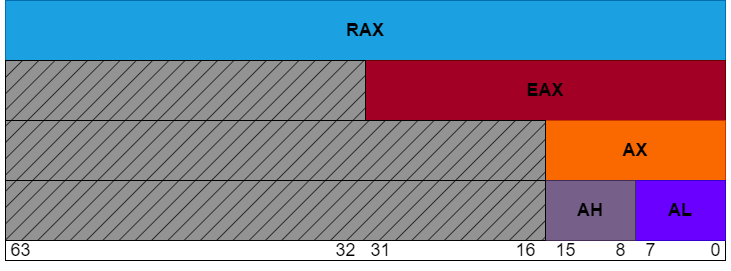
\includegraphics[width=\textwidth]{x64-register-layout.png}
        \column{0.5\textwidth}
        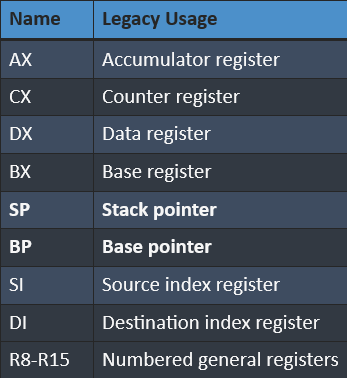
\includegraphics[scale=0.7]{x86-64_registers.png}
    \end{columns}
\end{frame}

\begin{frame}{Die shots}
    \begin{columns}
        \column{0.5\textwidth}
        Complete die intel tiger lake
        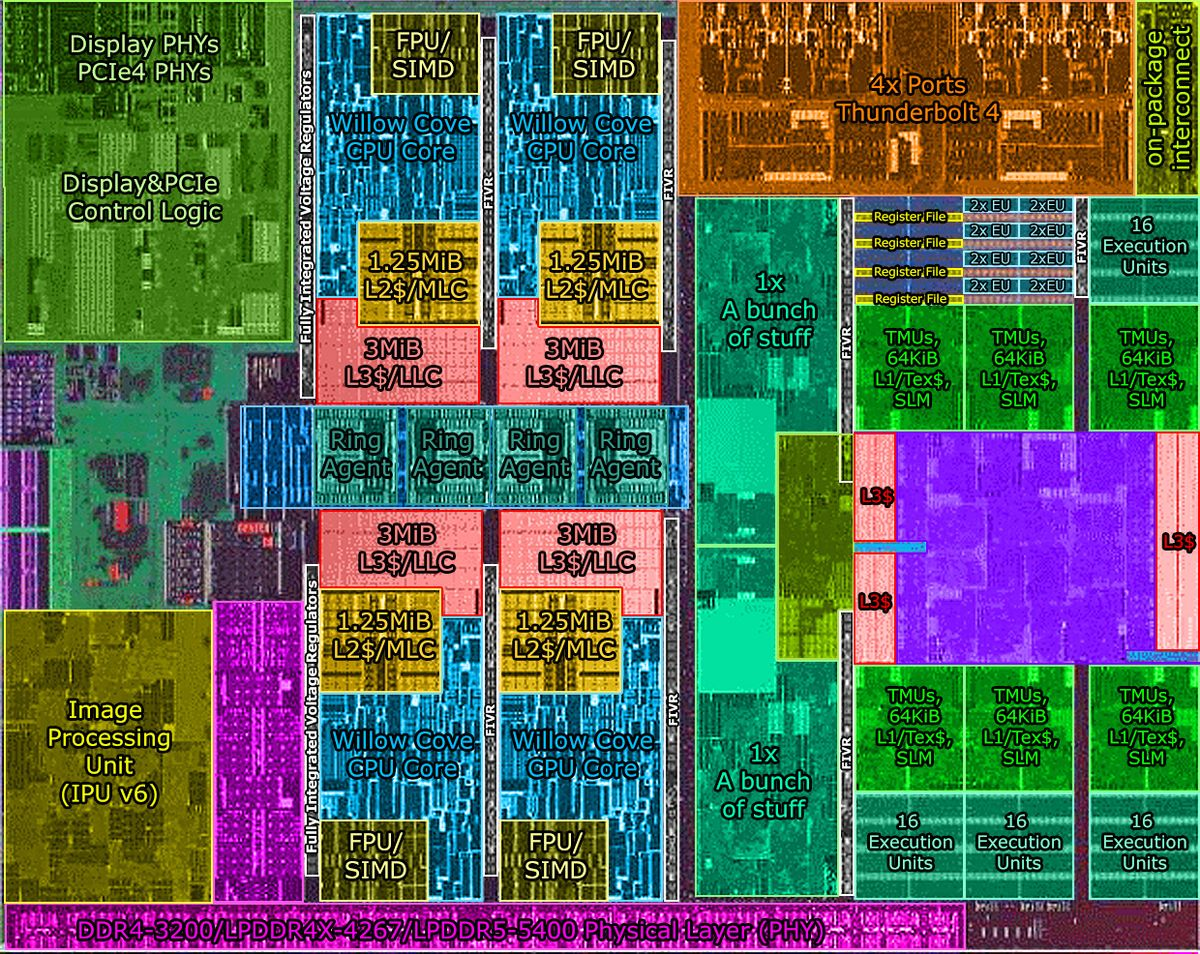
\includegraphics[scale = 0.17]{./images/tiger_lake_die_shot.jpg}
        source: \href{https://www.tomshardware.com/news/intel-details-tiger-lake-at-hot-chips-2020-die-revealed}{Intel tiger lake}
        \column{0.5\textwidth}
        Register closeup Z80
        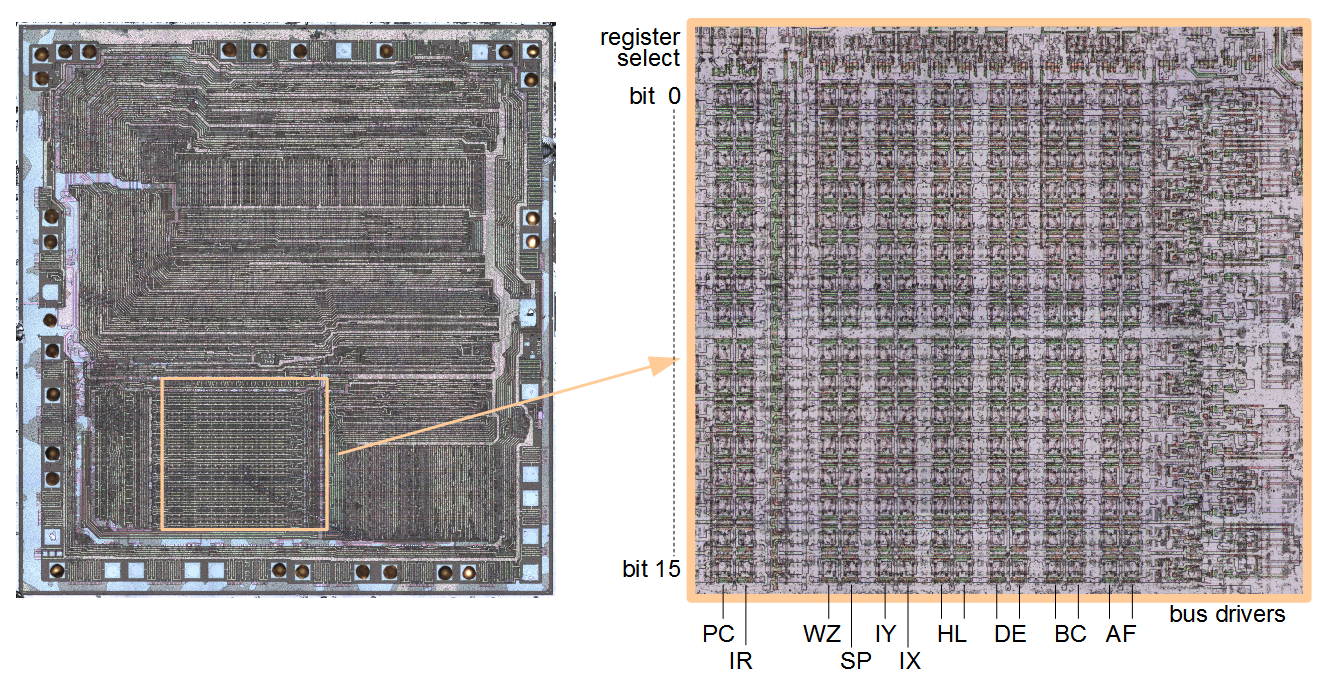
\includegraphics[scale = 0.17]{./images/die_register_zoom.png}3
        source: \href{https://www.righto.com/2014/10/how-z80s-registers-are-implemented-down.html}{Z80}
    \end{columns}
\end{frame}


\begin{frame}{Registers vs. memory}
    \begin{itemize}
        \item For assignments 1 and 3 we will use \textit{integer} registers
        \item Moving values between registers is extremely quick, a few clock-cycles
        \item Accessing \textit{memory} takes \textbf{hundreds}
        \item In the x86-64 ISA we are not allowed to move numbers directly between memory locations
        \item This means, you will have to utilize those registers!
    \end{itemize}

\end{frame}

\subsection{Assembly syntax}
\begin{frame}{Assembly syntax}{\sectiontitle}
    \begin{itemize}
        \item Two syntaxes are used for x86-64 assembly: \textit{Intel} and \textit{AT\&T/GAS}
        \item We will use \textbf{AT\&T}
        \item Be careful when looking up sources online, many will use the \textbf{Intel} syntax
        \item How do we know? AT\&T will use \textbf{\%} as a prefix for registers: \%rax
    \end{itemize}
    \begin{columns}
        \column{0.5\textwidth}
        \textbf{ATT}
        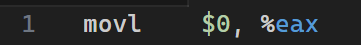
\includegraphics[width=\textwidth]{./images/att-register-access.png}
        \column{0.5\textwidth}
        \textbf{Intel}
        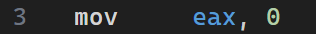
\includegraphics[width=\textwidth]{./images/intel-register-access.png}
    \end{columns}
\end{frame}

\subsection{Instructions}
\begin{frame}{Instructions}{\sectiontitle}
    \begin{itemize}
        \item There are many instructions in the x64(short for x86-64) ISA
        \item To begin with we will have a look at \textbf{INC}
        \item Inc increments the value of a target operand by '1'
        \item We can suffix the instruction with some letters to say what data size we are working with:
        \item \textit{b}: byte(1B), \textit{w}: word(2B), \textit{l}: long(4B), \textit{q}: quad(8B)
    \end{itemize}
\end{frame}

\begin{frame}{More instructions}{\sectiontitle}
    \begin{columns}
        \column{0.6\textwidth}
        \begin{itemize}
            \item \textit{DEC} Decrease value
            \item \textit{ADD} Add <src> to <dest>
            \item \textit{SUB} Subtract <src> from <dest>
            \item Immediate values are prefixed with \textit{\$}
            \item Comments start with \textit{\#}
        \end{itemize}
        \column{0.5\textwidth}
        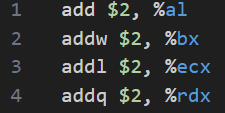
\includegraphics[]{./images/gas-att-add.png}
    \end{columns}
    \vspace{1cm}
    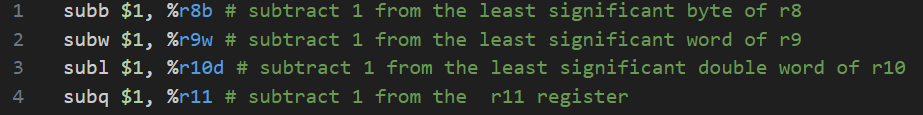
\includegraphics[scale=0.75]{./images/gas-att-sub.png}
\end{frame}


\begin{frame}{More Instructions}{\sectiontitle}
    \begin{itemize}
        \item \textit{MOV} move data; into a register, between two registers, or to memory
        \item \textbf{Remember} you cannot move data between two memory locations directly
    \end{itemize}
    \vspace{1cm}
    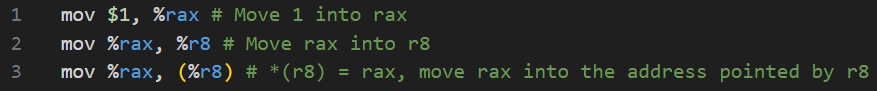
\includegraphics[width=\textwidth]{./images/gas-att-mov.png}
\end{frame}

\subsection{Pointers}
\begin{frame}{Pointers}{\sectiontitle}
    An important abstraction we know from previous courses is pointers. But in assembly they behave a bit different than in in the C language
    In \textbf{assembly} pointers:
    \begin{itemize}
        \item Does \textbf{not} increment by a multiple of the size of the data type it points to. This is perhaps more intuitive
              \begin{itemize}
                  \item ++ is \textbf{+1} not \textbf{+sizeof(type))}
              \end{itemize}
        \item We access pointers(memory addresses) by having parenthesis around a register whose value is the memory address, see previous slide
    \end{itemize}
\end{frame}

\subsection{Program flow}
\begin{frame}{Program flow}{\sectiontitle}
    \begin{itemize}
        \item Instructions are read \textbf{sequentially}
        \item The x86-ISA provides guarantees that instructions are executed \textbf{in-order}, meaning you will see the effect of instruction \textbf{1} before instruction \textbf{2} is executed
        \item This is not completely true, but a sufficient abstraction to have in mind for this course
        \item A special register called \textit{program counter}(PC) or \textit{instruction pointer}(IP) is used to keep track of the current instruction being executed
              \begin{itemize}
                  \item In x64 we call this register \textit{RIP}
                  \item The ISA does not allow us to access this register directly, but indirectly using jump instructions
              \end{itemize}
    \end{itemize}
\end{frame}

\begin{frame}{Program flow cont.}{\sectiontitle}
    \begin{itemize}
        \item Jump instructions break the sequential flow of programs
        \item In higher-level languages like C or Rust:
              \begin{itemize}
                  \item \textit{function calls}
                  \item \textit{loops}
                  \item \textit{conditional statements}
              \end{itemize}
        \item Translates into jump instructions
        \item In assembly we can define places to jump to using 'labels' (see next slide)
    \end{itemize}

\end{frame}

\begin{frame}{Jump}{\sectiontitle}
    \begin{itemize}
        \item We have two types of jump instructions: conditional or unconditional
        \item Unconditional jumps performs a jump to somewhere without any rules attached
        \item Conditional jumps on the other hand
              \begin{itemize}
                  \item Will check a so called \textit{flags}-register to determine if they should jump or continue to the sequential next instruction
                  \item There exist instructions to set these flags, and we will use the \textit{cmp}-family of instructions
              \end{itemize}
        \item This is enough to create \textit{if, loop,} etc.
    \end{itemize}

\end{frame}

\begin{frame}{Jump example}{\sectiontitle}
    \begin{columns}
        \column{0.5\textwidth}
        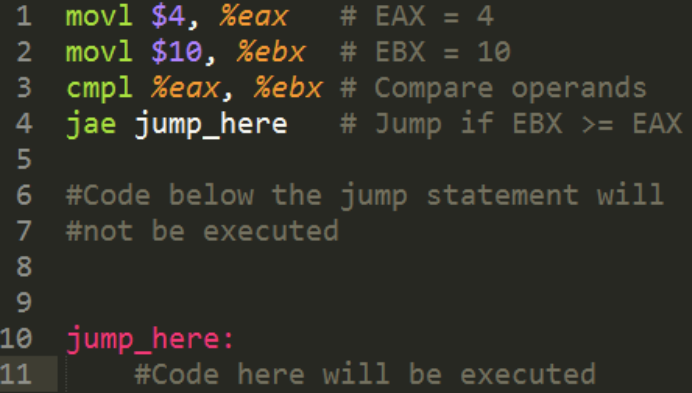
\includegraphics[scale=0.4]{./images/asm-cond-jmp.png}
        \column{0.5\textwidth}
        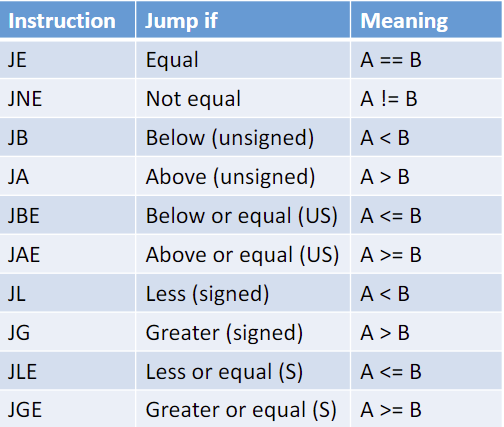
\includegraphics[scale=0.4]{./images/asm-jmp.png}
    \end{columns}
\end{frame}

\section{Stack}
\def \sectiontitle{Stack}
\begin{frame}{Stack}{\sectiontitle}
    \begin{columns}
        \column{0.5\textwidth}
        \begin{itemize}
            \item The hardware stack is memory that is accessed in a last-in-first-out manner
            \item In previous courses you have perhaps implemented software stacks, and it's exactly the same concept
            \item In x86 the stack 'grows' \textbf{downwards} in memory, from a high address to a low
        \end{itemize}

        source: \href{https://en.wikipedia.org/wiki/Stack-based_memory_allocation}{stack based memory}
        \column{0.5\textwidth}
        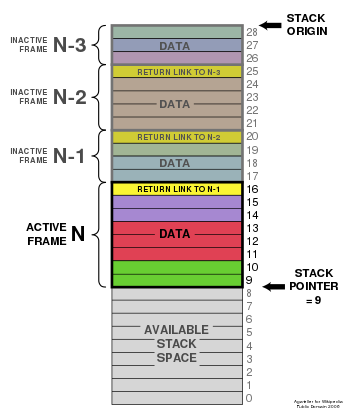
\includegraphics[scale=0.5]{./images/stack.png}
    \end{columns}
\end{frame}

\begin{frame}{Stack cont.}{\sectiontitle}
    \begin{itemize}
        \item In order to keep track of the stack we use two registers \textit{Stack pointer}(RSP), and \textit{Base pointer}(RBP)
        \item These two registers allows us to easily store
              \begin{itemize}
                  \item Function variables (local)
                  \item temporary data
                  \item functions arguments
              \end{itemize}
        \item That we would otherwise have to manually request memory for
    \end{itemize}
\end{frame}

\begin{frame}{Stack cont.}{\sectiontitle}
    \begin{itemize}
        \item The stack pointer(RSP) points to the 'top' of the stack, where we put a value last.
        \item Data below the stack pointer is considered garbage
        \item The base pointer(RBP) points to the 'bottom' of a so called \textit{stack-frame}.
        \item A stack frame is a portion of the total stack, and a local area for a particular function.
    \end{itemize}
\end{frame}

\begin{frame}{Stack cont.}{\sectiontitle}
    \begin{itemize}
        \item The x86-ISA defines two operations that makes working with the stack easier:
              \begin{itemize}
                  \item \textit{push}: Adds something to the stack
                  \item \textit{pop}: Removes something from the stack
              \end{itemize}
        \item The stack is currently 16-bit aligned, so there is no such thing as pushb/popb
        \item A good rule of thumb is to always keep symmetry between your pushes and pops
    \end{itemize}
\end{frame}

\begin{frame}{Stack cont.}{\sectiontitle}
    \begin{itemize}
        \item The stack operations affect the stack pointer(RSP), since it always points to the top of the stack
              \begin{itemize}
                  \item push will implicitly do: sub <size> rsp, mov <val> (\%rsp)
                  \item pop will implicitly do: add <size> rsp
              \end{itemize}
        \item You should not have to deal with endiannes, but worth noting:
              \begin{itemize}
                  \item The x86-family is \textit{little-endian}
              \end{itemize}
        \item If the register \textbf{EAX} has the value 0x012334567, and we want to move it into memory address 0xABCD0000
              \begin{itemize}
                  \item How will the four bytes that is the value of EAX be located in relation to the address?
              \end{itemize}
    \end{itemize}
\end{frame}

\subsection{Endianness}
\begin{frame}{Endianness}{\sectiontitle}
    Value: 0x01234567
    \begin{columns}
        \column{0.5\textwidth}
        \textbf{Big-endian}
        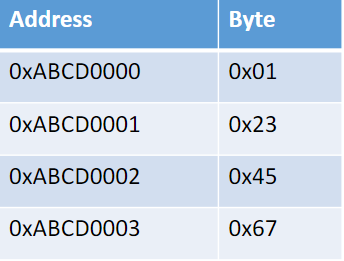
\includegraphics[width=\textwidth]{./images/big-endian.png}
        \column{0.5\textwidth}
        \textbf{Little-endian}
        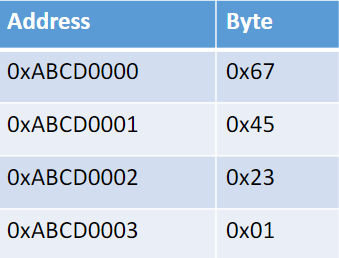
\includegraphics[width=\textwidth]{./images/little-endian.png}
        % TODO: Add new pictures

    \end{columns}

\end{frame}

\subsection{Stack pointer management}
\begin{frame}{Adding/subtracting on the stack pointer}{\sectiontitle}
    \begin{itemize}
        \item The stack pointer is constantly moving around, creating stack frames, pushing/poping values
        \item The base pointer is usually static after a new \textit{stack frame} has been set up
        \item To create a new stack frame:
              \begin{itemize}
                  \item Store the old value of the \textit{base pointer}
                  \item Copy the value of the \textit{stack pointer} into the base pointer
              \end{itemize}
        \item Voila! A new stack frame
        \item To clean up and return to the previous stack frame:
              \begin{itemize}
                  \item Pop up the stack / add to the stack pointer
                  \item Pop the stored base pointer value
              \end{itemize}
    \end{itemize}
\end{frame}

\section{Functions}
\def \sectiontitle {Functions}
\subsection{Calling convention}
\begin{frame}{Calling convention}{\sectiontitle}
    \begin{itemize}
        \item There exist different calling conventions. We will use \textbf{System V AMD64 ABI}
        \item This sets some rules for us when we call and create functions
        \item We divide our registers into two groups:
              \begin{itemize}
                  \item \textit{volatile}(caller-save/scratch)
                  \item \textit{non-volatile}(callee-saved)
              \end{itemize}
    \end{itemize}
\end{frame}

\begin{frame}{Calling convention cont.}{\sectiontitle}
    \begin{itemize}
        \item The caller-saved registers are:
              \begin{itemize}
                  \item RAX, RCX, RDX, R8, R9, R10, R11
              \end{itemize}
        \item The callee-saved registers are:
              \begin{itemize}
                  \item RBX, RBP, RDI, RSI, RSP, R12, R13, R14, R15
              \end{itemize}
    \end{itemize}
\end{frame}


\begin{frame}{Calling convention cont.}{\sectiontitle}
    \begin{itemize}
        \item The calling convention also specifies where return values should be put
        \item \textbf{RAX} is used for integer values up to 64-bit, for 128-bit integer values, RAX is combined with \textbf{RDX}
        \item There are more types of values
        \item For more details see: \url{https://www.uclibc.org/docs/psABI-x86_64.pdf}
    \end{itemize}

\end{frame}


\begin{frame}{Calling functions}{\sectiontitle}
    \begin{itemize}
        \item To call a function(label) in assembly we can use the \textbf{call} instruction
        \item This will save/push the \textit{instruction pointer} onto the stack
              \begin{itemize}
                  \item This means we can return to whereever we came from after a funtion is done
                  \item The function to 'undo' a call is called \textbf{ret}
              \end{itemize}
        \item This is why having symmetry and control over the stack pointer is so important, if we return and pop the wrong value for the instruction pointer, we will end up in weird places
    \end{itemize}
\end{frame}

\section{Examples}
\def \sectiontitle{examples}
\begin{frame}{Jumps}{\sectiontitle}
    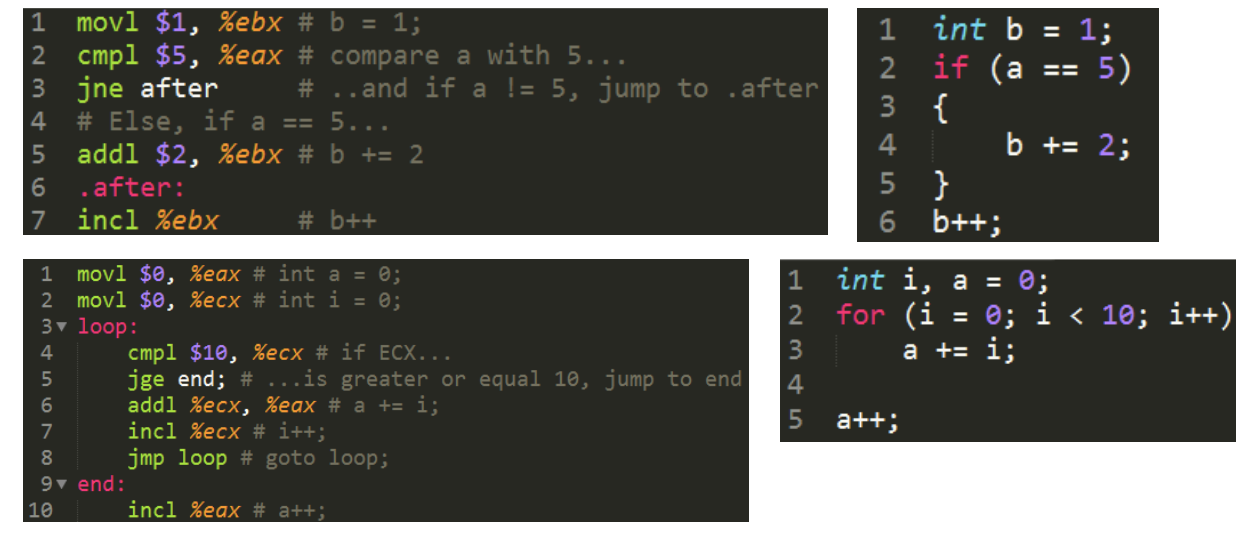
\includegraphics[scale=0.45]{./images/asm-program-examples.png}
\end{frame}

\section{Resources}
\def \sectiontitle{Resources}
\begin{frame}{Resources}
    \begin{itemize}
        \item \href{https://en.wikipedia.org/wiki/Moore\%27s_law}{Moore's law}
        \item \href{https://en.wikipedia.org/wiki/X86_calling_conventions\#System_V_AMD64_ABI}{Calling conventions}
        \item \href{https://en.wikibooks.org/wiki/X86_Assembly/GNU_assembly_syntax}{GAS assembly}
        \item \href{https://cs.brown.edu/courses/cs033/docs/guides/x64_cheatsheet.pdf}{x64 cheat sheet}
        \item \href{https://www.uclibc.org/docs/psABI-x86_64.pdf}{System V ABI}
        \item \href{https://learn.microsoft.com/en-us/windows-hardware/drivers/debugger/x64-architecture}{x64 registers}
        \item \href{https://godbolt.org}{Compiler explorer}
        \item \href{https://agner.org/}{Agner Fog's research (very,very good)}
    \end{itemize}

\end{frame}

\section{Q\&A}
\def \sectiontitle{Q\&A}
\begin{frame}{Q\&A}
    Questions?
\end{frame}


\end{document}
%----------------------------------------------------------------------------------------
